      
               
                \begin{ledgroupsized}[r]{120mm}
                \footnotesize 
                \pstart                
                \noindent\textbf{\"{U}berlieferung:}   
                \pend
                \end{ledgroupsized}
            
              
                            \begin{ledgroupsized}[r]{114mm}
                            \footnotesize 
                            \pstart \parindent -6mm
                            \makebox[6mm][l]{\textit{L}}Notiz: LH XXXV 12, 2 Bl. 62. 1 Bl. 4\textsuperscript{o}. \nicefrac{1}{2} S. auf Bl.~62~r\textsuperscript{o}. In der unteren Hälfte von Bl.~62~r\textsuperscript{o} Rechnungen, die in \textit{LSB} VII,~3 N.~38\textsubscript{16} ediert sind; Bl.~62~v\textsuperscript{o} überliefert das Stück \textit{LSB} VII,~5 N.~9. Ein Wasserzeichen, beschnitten. Papier durch Erhaltungsmaßnahmen stabilisiert.%
\newline%
Cc 2, Nr. 543 (tlw.)%
\pend%
%                            Konzept: LH XXXV 12, 2 Bl. 62. 1 Bl. 4\textsuperscript{o}. Papier durch Erhaltungs\-ma{\ss}nahmen stabilisiert. \nicefrac{1}{2} S. auf Bl. 62~r\textsuperscript{o}. Wasserzeichen beschnitten. In der unteren Hälfte von Bl. 62~r\textsuperscript{o} Rechnungen, die in \cite{00115}\title{LSB} VII, 3 N. 38.16 ediert sind; Bl. 62~v\textsuperscript{o} enthält das Stück \cite{00115}\title{LSB} VII, 5 N. 9.\\Cc 2, Nr. 543 \pend
                            \end{ledgroupsized}
                %\normalsize
                \vspace*{5mm}
                \begin{ledgroup}
                \footnotesize 
                \pstart
            \noindent\footnotesize{\textbf{Datierungsgr\"{u}nde}: Die Datierung des St\"{u}ckes folgt derjenigen, die f\"{u}r \title[115]{LSB} VII, 5 N. 9 geliefert wird, und der dort geäußerten Vermutung, dass Leibniz zuerst die mathematischen Aufzeich\-nungen auf der R\"{u}ckseite von Bl. 62 verfasst habe. Das vorliegende St\"{u}ck k\"{o}nnte daher gleichfalls im Oktober 1674 oder in den folgenden Monaten entstanden sein, wie das Wasserzeichen nahelegt.}
                \pend
                \end{ledgroup}
            
                \vspace*{8mm}
                \pstart 
                \normalsize
            \noindent[62~r\textsuperscript{o}]  Pendulorum longitudines duplicatam habent rationem temporum, quibus minimae vibrationes\protect\index{Sachverzeichnis}{vibratio} perficiuntur.\pend \pstart \vspace{2em} \noindent
\begin{minipage}[t]{0.33\textwidth}
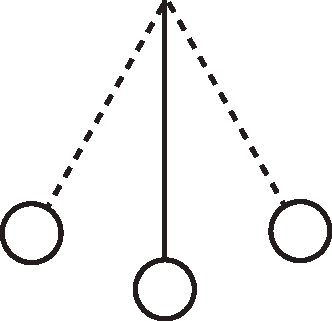
\includegraphics[width=0.6\textwidth]{images/62-1.pdf}
\end{minipage}
\hspace*{13,3mm}
\begin{minipage}[t]{0.33\textwidth}
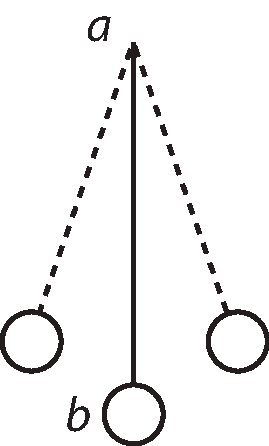
\includegraphics[width=0.47\textwidth]{images/62-2.pdf}
\end{minipage}
\hspace*{13,3mm}
\begin{minipage}[t]{0.33\textwidth}

\includegraphics[width=0.18\textwidth]{images/62_3.pdf}
\end{minipage}

%\begin{center}                    
            %   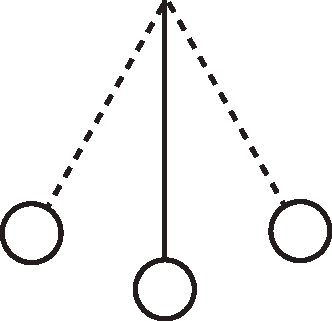
\includegraphics[width=0.55\textwidth]{images/62-1.pdf}
             %  \end{center}
               \vspace*{1mm}
                    \hspace*{-1,5mm}  [\textit{Fig. 1}]\hspace*{44mm}  [\textit{Fig. 2}] \hspace*{38mm}  [\textit{Fig. 3, gestr.}]
\vspace*{1em}                       
                        %@ @ @ Dies ist eine Abstandszeile - fuer den Fall, dass mehrere figures hintereinander kommen, ohne dass dazwischen laengerer Text steht. Dies kann zu einer Fahlermeldung fuehren. @ @ @ \\
                   
                    \vspace{2em} \noindent \setline{13}\lbrack \textit{Rechnungsfragmente ohne Textbezug:}\rbrack \pend
\vspace{1em}
                     \pstart \noindent 
 \begin{tabular}{c}
                                   1500\\
                                   1000\\
                                  \end{tabular}
                        %@ @ @ Dies ist eine Abstandszeile - fuer den Fall, dass mehrere figures hintereinander kommen, ohne dass dazwischen laengerer Text steht. Dies kann zu einer Fahlermeldung fuehren. @ @ @ \\
                    \begin{tabular}{cc}
                                  999 &333\\
                                 \end{tabular}
                        %@ @ @ Dies ist eine Abstandszeile - fuer den Fall, dass mehrere figures hintereinander kommen, ohne dass dazwischen laengerer Text steht. Dies kann zu einer Fahlermeldung fuehren. @ @ @ \\
                     \pend 
 


 


 


 


 

